% =============================================================================
% Appendix: FESTIM-NIUQ Package Documentation
% =============================================================================
% Draft version — see Section~\ref{sec:questions} for open questions.
% Compile with: pdflatex appendix_festim_niuq.tex  (twice for references)
% Requires: TeX Live 2020 or later (for modern TikZ libraries)
% =============================================================================
\documentclass[11pt,a4paper]{article}

% ---------- packages --------------------------------------------------------
\usepackage[utf8]{inputenc}
\usepackage[T1]{fontenc}
\usepackage{lmodern}
\usepackage[margin=2.5cm]{geometry}
\usepackage{amsmath,amssymb}
\usepackage{booktabs}
\usepackage{longtable}
\usepackage{array}
\usepackage{tabularx}
\usepackage{xcolor}
\usepackage{hyperref}
\usepackage{tikz}
\usetikzlibrary{
  shapes.geometric,
  arrows.meta,
  positioning,
  fit,
  calc,
  backgrounds,
  decorations.pathreplacing
}
\usepackage{listings}
\usepackage{caption}

% ---------- custom colours --------------------------------------------------
\definecolor{festimblue}{HTML}{2B6CB0}
\definecolor{uqgreen}{HTML}{38A169}
\definecolor{toolorange}{HTML}{DD6B20}
\definecolor{lightgray}{HTML}{F7FAFC}
\definecolor{codebg}{HTML}{EDF2F7}

% ---------- listings style --------------------------------------------------
\lstset{
  basicstyle=\ttfamily\small,
  backgroundcolor=\color{codebg},
  frame=single,
  framerule=0.4pt,
  rulecolor=\color{gray!50},
  breaklines=true,
  columns=fullflexible,
}

% ---------- TikZ styles -----------------------------------------------------
\tikzstyle{classbox} = [
  rectangle, rounded corners=3pt, draw=festimblue, thick,
  fill=festimblue!8, text width=4.2cm, minimum height=1.1cm,
  align=center, font=\small\sffamily
]
\tikzstyle{utilbox} = [
  rectangle, rounded corners=3pt, draw=uqgreen, thick,
  fill=uqgreen!8, text width=3.8cm, minimum height=1cm,
  align=center, font=\small\sffamily
]
\tikzstyle{scriptbox} = [
  rectangle, rounded corners=3pt, draw=toolorange, thick,
  fill=toolorange!8, text width=4cm, minimum height=1cm,
  align=center, font=\small\sffamily
]
\tikzstyle{extbox} = [
  rectangle, rounded corners=3pt, draw=gray, thick,
  fill=gray!8, text width=3.2cm, minimum height=0.9cm,
  align=center, font=\small\sffamily
]
\tikzstyle{flowbox} = [
  rectangle, rounded corners=4pt, draw=festimblue!80, thick,
  fill=festimblue!10, text width=3.6cm, minimum height=1.1cm,
  align=center, font=\small\sffamily
]
\tikzstyle{decisionbox} = [
  diamond, draw=toolorange!80, thick,
  fill=toolorange!10, text width=2.2cm,
  align=center, font=\small\sffamily, aspect=2
]
\tikzstyle{arrowstyle} = [-{Stealth[length=3mm]}, thick]

% ---------- title -----------------------------------------------------------
\title{%
  \textbf{Appendix: FESTIM-NIUQ Package}\\[4pt]
  \large Non-Intrusive Uncertainty Quantification\\
  for Tritium Transport Simulations%
}
\author{FESTIM-NIUQ Development Team}
\date{Draft — \today}

\begin{document}
\maketitle
\tableofcontents
\newpage

% ============================================================================
\section{Introduction}
\label{sec:intro}
% ============================================================================

FESTIM-NIUQ is a Python package that performs \emph{non-intrusive uncertainty
quantification} (NIUQ) for tritium transport simulations built with the
\href{https://github.com/festim-dev/FESTIM}{FESTIM} finite-element code.
The package relies on
\href{https://github.com/UCL-CCS/EasyVVUQ}{EasyVVUQ} (part of the SEAVEA
Toolkit) to orchestrate parametric sampling, surrogate construction, and
sensitivity analysis, while the deterministic forward model is driven by
FESTIM~v1.4 and v2.0.

The principal capabilities are:
\begin{itemize}
  \item Forward uncertainty propagation via Polynomial Chaos Expansion (PCE)
        and quasi-Monte~Carlo (QMC) sampling.
  \item Correlated parameter uncertainty propagation using multivariate
        normal distributions and finite-difference (FD) or PCE samplers.
  \item Covariance influence analysis — scanning correlation coefficients
        and tracking Sobol indices.
  \item Postprocessing, interactive visualisation, and statistics logging.
\end{itemize}


% ============================================================================
\section{Physical Model}
\label{sec:physics}
% ============================================================================

The underlying physics modelled by FESTIM describes the transport and
retention of hydrogen isotopes (primarily \emph{tritium}) in solid
materials exposed to a tritium source. The governing partial differential
equations solved in the 1-D domain $\Omega = [0, L]$ are:

\subsection{Tritium Transport (Hydrogen Diffusion)}

The tritium concentration $c(\mathbf{r}, t)$ obeys a diffusion--source
equation:
\begin{equation}
  \frac{\partial c}{\partial t}
  = \nabla \cdot \bigl( D(T)\,\nabla c \bigr) + G,
  \label{eq:diffusion}
\end{equation}
where $G$ $\mathrm{[m^{-3}\,s^{-1}]}$ is the volumetric tritium generation
rate and the temperature-dependent diffusivity follows an Arrhenius law:
\begin{equation}
  D(T) = D_0 \exp\!\Bigl(-\frac{E_D}{k_B T}\Bigr).
  \label{eq:arrhenius}
\end{equation}

\subsection{Heat Transfer}

When coupled heat transfer is enabled, the temperature field $T(\mathbf{r},t)$
satisfies:
\begin{equation}
  \rho \, c_p \frac{\partial T}{\partial t}
  = \nabla \cdot \bigl(\kappa \,\nabla T\bigr) + Q,
  \label{eq:heat}
\end{equation}
where $\rho$ is the material density, $c_p$ is the specific heat capacity,
$\kappa$ is the thermal conductivity, and $Q$ $\mathrm{[W\,m^{-3}]}$ is a
volumetric heat source.

\subsection{Boundary Conditions}

The code supports:
\begin{itemize}
  \item \textbf{Dirichlet:} $c\big|_{\partial\Omega} = c_0$ \; or \;
        $T\big|_{\partial\Omega} = T_0$.
  \item \textbf{Neumann (flux):} $-D\,\nabla c \cdot \hat{n} = J_0$ \; or \;
        $-\kappa\,\nabla T \cdot \hat{n} = q_0$.
  \item \textbf{Convective flux:}
        $-\kappa\,\nabla T \cdot \hat{n} = h_\mathrm{conv}(T - T_\mathrm{ext})$.
  \item \textbf{Surface recombination:}
        $J_\mathrm{rec} = k_{r0}\,\exp(-E_{k_r}/k_B T)\,c^2$ (where applicable).
\end{itemize}

\subsection{Coordinate Systems}

The 1-D domain can be interpreted in Cartesian, cylindrical, or spherical
coordinates.  In spherical symmetry the Laplacian takes the form
\begin{equation}
  \nabla^2 c = \frac{1}{r^2}\frac{\partial}{\partial r}
               \Bigl(r^2 \frac{\partial c}{\partial r}\Bigr),
\end{equation}
which modifies the volume-integration weights used when computing integral
quantities (e.g.\ tritium inventory).

\subsection{Quantities of Interest}

From the solution fields, the package computes:
\begin{itemize}
  \item \textbf{Tritium inventory:}
        $\displaystyle I(t) = \int_\Omega c(\mathbf{r},t)\,\mathrm{d}V$.
  \item \textbf{Total tritium release} via mass balance:
        $R(t) = I(0) + \int_0^t G\,\mathrm{d}V\,\mathrm{d}t' - I(t)$.
\end{itemize}


% ============================================================================
\section{Main Classes and Functions}
\label{sec:classes}
% ============================================================================

\subsection{FESTIM Model Layer (\texttt{festim\_model/})}

\begin{description}
  \item[\texttt{BaseModel}] Abstract base class declaring the interface for
    all FESTIM model wrappers.  Virtual methods include
    \texttt{\_specify\_geometry}, \texttt{\_specify\_materials},
    \texttt{\_specify\_boundary\_conditions}, \texttt{\_add\_source\_terms},
    \texttt{\_add\_heat\_conduction}, \texttt{\_specify\_time\_integration\_settings},
    \texttt{\_add\_derived\_quantities}, and \texttt{run}.

  \item[\texttt{Model\_legacy}] Concrete wrapper for FESTIM~v1.4.  Reads a
    YAML configuration, builds a \texttt{festim.Simulation} object (geometry,
    materials, BCs, sources, time stepping, exports), and runs it.
    Outputs \texttt{TXTExport} profile data.

  \item[\texttt{Model}] Concrete wrapper for FESTIM~v2.0.  Supports
    multiple coupled problems (\texttt{HydrogenTransportProblem},
    \texttt{HeatTransferProblem}), FESTIM~2.0 mesh types (\texttt{Mesh1D}),
    species objects, and milestone-time profile exports via the custom
    \texttt{ProfileExport} class.
    Key methods:
    \begin{itemize}
      \item \texttt{\_specify\_geometry}: Creates 1-D meshes with optional
            local refinement (linear or quadratic rules).
      \item \texttt{\_specify\_materials}: Parses material list from YAML,
            constructs \texttt{festim.Material} objects with $D_0$, $E_D$,
            $\kappa$, $\rho$, $c_p$.
      \item \texttt{\_specify\_boundary\_conditions}: Maps YAML BC specs to
            FESTIM BC objects (Dirichlet, Neumann, convective, recombination).
      \item \texttt{\_export\_results}: Extracts milestone profiles from
            \texttt{ProfileExport.data}, saves CSV for the UQ decoder,
            computes total tritium release via mass balance.
      \item \texttt{run}: Initialises, solves, and exports.
    \end{itemize}

  \item[\texttt{ProfileExport}] Subclass of \texttt{festim.VolumeQuantity}
    that appends the full concentration array after every solve step
    for later milestone extraction.

  \item[\texttt{Diagnostics}] Postprocessing class that reads simulation
    results (TXT or BP/VTX format), computes derived quantities
    (e.g.\ tritium inventory), and generates visualisation plots.
\end{description}


\subsection{UQ Orchestration Layer (\texttt{uq/})}

\begin{description}
  \item[\texttt{easyvvuq\_festim.py}]
    Stand-alone forward-UQ driver for \emph{independent} parameters.
    Provides:
    \begin{itemize}
      \item \texttt{define\_parameter\_uncertainty(config, CoV, distribution)}:
            Builds \texttt{chaospy} distributions from YAML means and CoVs.
      \item \texttt{define\_festim\_model\_parameters()}: Returns the
            parameter dictionary and QoI column list for EasyVVUQ.
      \item \texttt{prepare\_uq\_campaign(config, \dots)}: Assembles encoder,
            decoder, execution action, sampler (PCE or QMC), and campaign.
      \item \texttt{run\_uq\_campaign(campaign, pool)}: Executes the
            campaign with a QCG-PJ resource pool.
      \item \texttt{analyse\_uq\_results}: Runs PCE or QMC analysis and
            returns statistical results.
      \item \texttt{visualisation\_of\_results}: Generates uncertainty and
            Sobol-index plots.
    \end{itemize}

  \item[\texttt{easyvvuq\_festim\_correlated.py}]
    Forward-UQ driver for \emph{correlated} parameters.  Constructs a
    multivariate normal distribution
    (\texttt{chaospy.MvNormal}) from per-parameter CoVs and an
    inter-parameter correlation coefficient.
    Supports FD and PCE samplers.

  \item[\texttt{covariance\_influence\_analysis.py}]
    Scans a range of correlation coefficient values (log or linear scale),
    runs a correlated PCE campaign at each, and collects first-order and
    total Sobol indices.  Results are saved as CSV, JSON, and PDF plots.

  \item[\texttt{festim\_model\_run.py}]
    Thin wrapper executed by EasyVVUQ for each sample.  Loads a YAML
    config, instantiates \texttt{Model} or \texttt{Model\_legacy},
    runs the simulation, and writes \texttt{output.csv} with scalar QoIs.

  \item[\texttt{uq\_postprocessing.py}]
    Standalone postprocessing that reloads a completed campaign (from
    database, pickle, or run directory) and regenerates plots and
    statistics logs.

  \item[\texttt{interactive\_run\_viewer.py}]
    Generates a self-contained HTML+Plotly.js viewer from an EasyVVUQ
    campaign's run directories, with dropdown selectors for each
    uncertain parameter.
\end{description}


\subsection{Utility Modules (\texttt{uq/util/})}

\begin{description}
  \item[\texttt{Encoder.py}]
    \texttt{YAMLEncoder} — simple delimiter-based substitution;
    \texttt{AdvancedYAMLEncoder} — dot-notation path-based YAML
    manipulation that directly modifies nested YAML keys (e.g.\
    \texttt{materials.D\_0.mean}).

  \item[\texttt{Decoder.py}]
    \texttt{ScalarCSVDecoder} — reads single-row CSV files containing
    scalar QoIs (\texttt{output.csv}) for Bayesian inversion campaigns.

  \item[\texttt{plotting.py}]
    \texttt{UQPlotter} class with methods such as
    \texttt{plot\_unc\_vs\_r}, \texttt{plot\_stats\_vs\_r},
    \texttt{plot\_stats\_correlated}, and Sobol-index bar charts.
    Uses \texttt{matplotlib} with the \texttt{Agg} backend for headless
    servers.

  \item[\texttt{utils.py}]
    Shared helpers: \texttt{load\_config}, \texttt{add\_timestamp\_to\_filename},
    \texttt{get\_festim\_python}, \texttt{validate\_execution\_setup}.
\end{description}


% ============================================================================
\section{Numerical Parameters}
\label{sec:parameters}
% ============================================================================

Table~\ref{tab:params} lists the uncertain numerical parameters supported
by the UQ campaigns.  Mean values are read from the YAML configuration
file; distributions and coefficients of variation are set at run-time.

\begin{table}[htbp]
\centering
\caption{Numerical parameters considered in FESTIM-NIUQ uncertainty quantification.}
\label{tab:params}
\footnotesize
\setlength{\tabcolsep}{4pt}
\begin{tabularx}{\textwidth}{@{} l l l X @{}}
\toprule
\textbf{Symbol} & \textbf{Name} & \textbf{Unit} & \textbf{Description / YAML key} \\
\midrule
$D_0$         & Diffusion coefficient       & $\mathrm{m^2\,s^{-1}}$      & Pre-exponential Arrhenius diffusivity \newline \texttt{materials.D\_0.mean} \\[2pt]
$E_D$         & Activation energy           & $\mathrm{eV}$               & Activation energy for diffusion \newline \texttt{materials.E\_D.mean} \\[2pt]
$\kappa$      & Thermal conductivity        & $\mathrm{W\,m^{-1}K^{-1}}$  & Thermal conductivity \newline \texttt{materials.thermal\_conductivity.mean} \\[2pt]
$\rho$        & Density                     & $\mathrm{kg\,m^{-3}}$       & Material density \newline \texttt{materials.rho.mean} \\[2pt]
$c_p$         & Heat capacity               & $\mathrm{J\,kg^{-1}K^{-1}}$ & Specific heat capacity \newline \texttt{materials.heat\_capacity.mean} \\[2pt]
$G$           & Generation rate             & $\mathrm{m^{-3}\,s^{-1}}$   & Volumetric tritium generation rate \newline \texttt{source\_terms.concentration.value.mean} \\[2pt]
$Q$           & Heat source                 & $\mathrm{W\,m^{-3}}$        & Volumetric heat source \newline \texttt{source\_terms.heat.value.mean} \\[2pt]
$E_{k_r}$     & Recombination energy        & $\mathrm{eV}$               & Surface recomb.\ activation energy \newline \texttt{boundary\_conditions\ldots E\_kr.mean} \\[2pt]
$k_{r0}$      & Recomb.\ rate constant      & $\mathrm{m\,s^{-1}}$        & Pre-exponential recombination constant \\[2pt]
$h_\mathrm{conv}$ & Convective HT coeff.   & $\mathrm{W\,m^{-2}K^{-1}}$  & Boundary convective heat-transfer coeff.\ \newline \texttt{boundary\_conditions\ldots h\_conv.mean} \\[2pt]
$E_k$         & Trapping energy             & $\mathrm{eV}$               & Trapping energy (Boltzmann weighting) \newline \texttt{materials.E\_k.mean} \\
\bottomrule
\end{tabularx}
\end{table}

\noindent
Table~\ref{tab:sim_params} lists the main simulation (numerical) settings.

\begin{table}[htbp]
\centering
\caption{Simulation control parameters.}
\label{tab:sim_params}
\small
\begin{tabularx}{\textwidth}{@{} l l X @{}}
\toprule
\textbf{Parameter} & \textbf{Default} & \textbf{Description} \\
\midrule
\texttt{n\_elements}        & 128--1024   & Number of finite elements in the 1-D mesh \\
\texttt{mesh\_type}         & \texttt{regular} & Mesh type: \texttt{regular} or \texttt{refined} (quadratic / linear rule) \\
\texttt{time\_step}         & 0.01\,s     & Initial (or fixed) time step for transient runs \\
\texttt{max\_stepsize}      & 0.1\,s      & Maximum adaptive time step \\
\texttt{stepsize\_change\_ratio} & 1.1    & Ratio for adaptive time-stepping \\
\texttt{absolute\_tolerance}& $10^{6}$    & Absolute solver tolerance (problem-specific) \\
\texttt{relative\_tolerance}& $10^{-6}$   & Relative solver tolerance \\
\texttt{total\_time}        & ---         & Final simulation time (transient only) \\
\texttt{milestone\_times}   & [list]      & Checkpoint times for profile export \\
\bottomrule
\end{tabularx}
\end{table}


% ============================================================================
\section{Quantities of Interest (QoIs)}
\label{sec:qois}
% ============================================================================

\begin{table}[htbp]
\centering
\caption{Quantities of interest measured and analysed in FESTIM-NIUQ.}
\label{tab:qois}
\small
\begin{tabularx}{\textwidth}{@{} l l l X @{}}
\toprule
\textbf{QoI} & \textbf{Type} & \textbf{Unit} & \textbf{Description} \\
\midrule
Tritium concentration $c(r,t)$   & Profile (1-D)   & $\mathrm{m^{-3}}$   & Spatial profile of the mobile tritium concentration at each milestone time \\
Temperature $T(r,t)$             & Profile (1-D)   & K                    & Temperature distribution (when heat transfer is coupled) \\
Tritium inventory $I(t)$         & Scalar / series  & (see note$^\ast$) & Volume-integrated tritium content: $I = \int_\Omega c\,\mathrm{d}V$ \\
Total tritium release $R(t)$     & Scalar / series  & ---                  & Cumulative release via mass balance: $R = I_0 + \int_0^t G\,\mathrm{d}V\,\mathrm{d}t' - I$ \\
Total tritium trapping           & Scalar           & ---                  & Trapped fraction via Boltzmann weighting with $E_k$ \\
\bottomrule
\end{tabularx}
\end{table}

\noindent
$^\ast$\textit{Note:} The unit of tritium inventory depends on the
concentration unit and domain volume.  If $c$ is in
$\mathrm{m^{-3}}$ (number density), then
$I = \int c\,\mathrm{d}V$ is a total count (dimensionless).
This should be clarified for the specific application., the EasyVVUQ decoder reads columns named
\texttt{t=\textit{time}s} from \texttt{results\_tritium\_concentration.txt}.
For steady-state runs the column is \texttt{t=steady}.
Scalar QoIs are written to \texttt{output.csv}.

% ============================================================================
\section{Code Architecture Diagram}
\label{sec:arch}
% ============================================================================

Figure~\ref{fig:architecture} shows the high-level module architecture.

\begin{figure}[htbp]
\centering
\resizebox{\textwidth}{!}{%
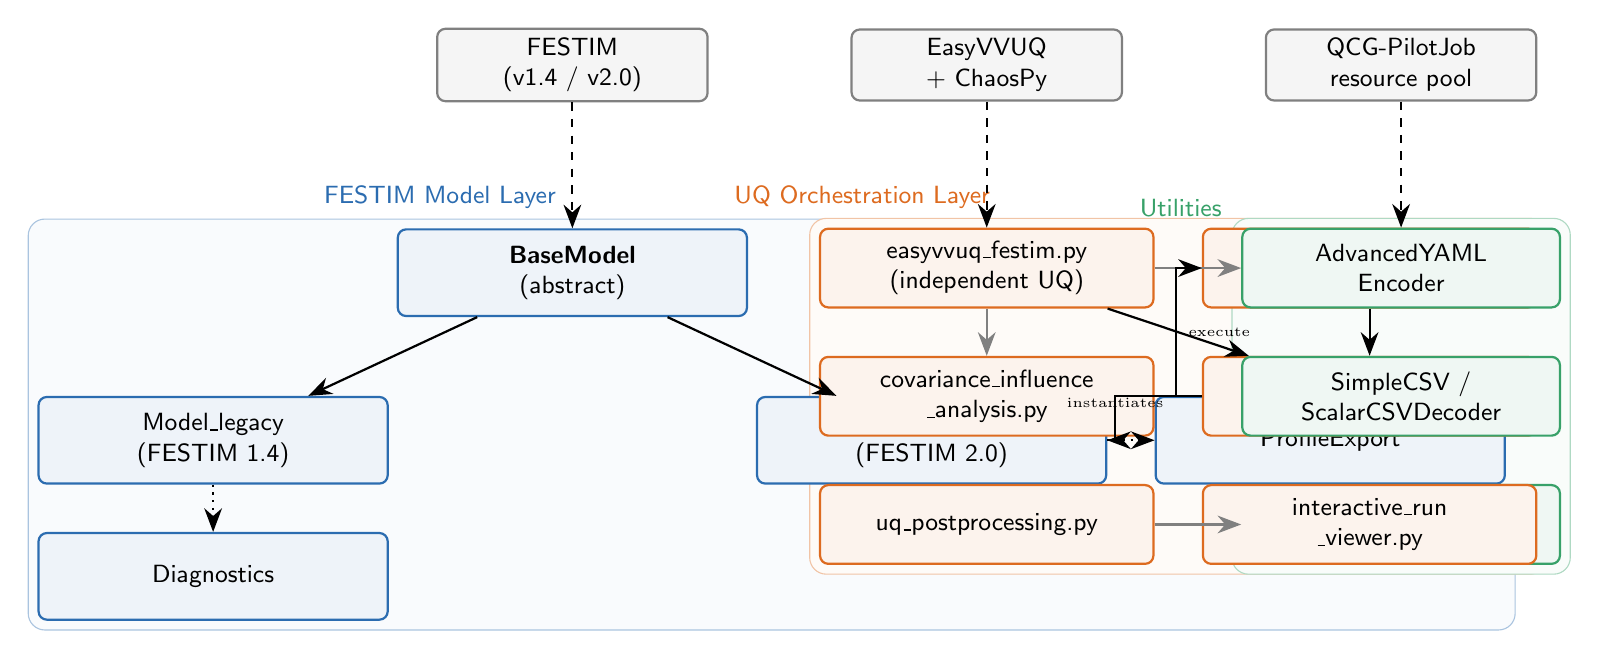
\begin{tikzpicture}[node distance=1.2cm and 1.4cm]

% --- External dependencies ---
\node[extbox] (festim) {FESTIM\\(v1.4 / v2.0)};
\node[extbox, right=1.8cm of festim] (easyvvuq) {EasyVVUQ\\+ ChaosPy};
\node[extbox, right=1.8cm of easyvvuq] (qcgpj) {QCG-PilotJob\\resource pool};

% --- FESTIM model layer ---
\node[classbox, below=1.6cm of festim] (basemodel) {\textbf{BaseModel}\\(abstract)};
\node[classbox, below left=1.0cm and 0.1cm of basemodel] (legacy) {Model\_legacy\\(FESTIM 1.4)};
\node[classbox, below right=1.0cm and 0.1cm of basemodel] (model) {\textbf{Model}\\(FESTIM 2.0)};
\node[classbox, right=0.6cm of model] (profexp) {ProfileExport};
\node[classbox, below=0.6cm of legacy] (diag) {Diagnostics};

% --- UQ layer ---
\node[scriptbox, below=1.6cm of easyvvuq] (uqind) {easyvvuq\_festim.py\\(independent UQ)};
\node[scriptbox, right=0.6cm of uqind] (uqcorr) {easyvvuq\_festim\\\_correlated.py};
\node[scriptbox, below=0.6cm of uqind] (covana) {covariance\_influence\\\_analysis.py};
\node[scriptbox, below=0.6cm of uqcorr] (fmrun) {festim\_model\_run.py\\(per-sample wrapper)};

% --- Utilities ---
\node[utilbox, below=1.6cm of qcgpj] (encoder) {AdvancedYAML\\Encoder};
\node[utilbox, below=0.6cm of encoder] (decoder) {SimpleCSV /\\ScalarCSVDecoder};
\node[utilbox, below=0.6cm of decoder] (plotter) {UQPlotter};

% --- Post-processing ---
\node[scriptbox, below=0.6cm of covana] (postproc) {uq\_postprocessing.py};
\node[scriptbox, right=0.6cm of postproc] (viewer) {interactive\_run\\\_viewer.py};

% --- Arrows ---
\draw[arrowstyle, dashed] (festim) -- (basemodel);
\draw[arrowstyle, dashed] (easyvvuq) -- (uqind);
\draw[arrowstyle, dashed] (qcgpj) -- (encoder);

\draw[arrowstyle] (basemodel) -- (legacy);
\draw[arrowstyle] (basemodel) -- (model);

\draw[arrowstyle, dotted] (model) -- (profexp);
\draw[arrowstyle, dotted] (legacy) -- (diag);

\draw[arrowstyle] (uqind) -- (fmrun) node[midway, right, font=\tiny] {execute};
\draw[arrowstyle] (uqcorr) -- (fmrun);
\draw[arrowstyle] (fmrun.west) -- +(-1.1,0) |- (model.east) node[near start, above, font=\tiny] {instantiates};

\draw[arrowstyle, gray] (uqind.east) -- ++(0.2,0) |- (encoder.west);
\draw[arrowstyle, gray] (uqind) -- (covana);
\draw[arrowstyle, gray] (postproc) -- (plotter.west |- postproc);

\draw[arrowstyle] (covana) -- ++(2.4,0) |- (uqcorr);

% --- Background boxes ---
\begin{scope}[on background layer]
  \node[draw=festimblue!40, fill=festimblue!3, rounded corners=6pt,
        fit=(basemodel)(legacy)(model)(profexp)(diag),
        label={[festimblue, font=\sffamily\small]above left:FESTIM Model Layer}] {};
  \node[draw=toolorange!40, fill=toolorange!3, rounded corners=6pt,
        fit=(uqind)(uqcorr)(covana)(fmrun)(postproc)(viewer),
        label={[toolorange, font=\sffamily\small]above left:UQ Orchestration Layer}] {};
  \node[draw=uqgreen!40, fill=uqgreen!3, rounded corners=6pt,
        fit=(encoder)(decoder)(plotter),
        label={[uqgreen, font=\sffamily\small]above left:Utilities}] {};
\end{scope}

\end{tikzpicture}%
}
\caption{High-level architecture of the FESTIM-NIUQ package.
  Blue boxes: FESTIM model layer; orange boxes: UQ orchestration scripts;
  green boxes: utility modules; grey boxes: external dependencies.
  Solid arrows denote calls or inheritance; dashed arrows denote
  dependency on external libraries; dotted arrows denote composition.}
\label{fig:architecture}
\end{figure}


% ============================================================================
\section{Typical UQ Workflow}
\label{sec:workflow}
% ============================================================================

Figure~\ref{fig:workflow} illustrates the typical uncertainty-quantification
workflow from configuration to results.

\begin{figure}[htbp]
\centering
\resizebox{0.72\textwidth}{!}{%
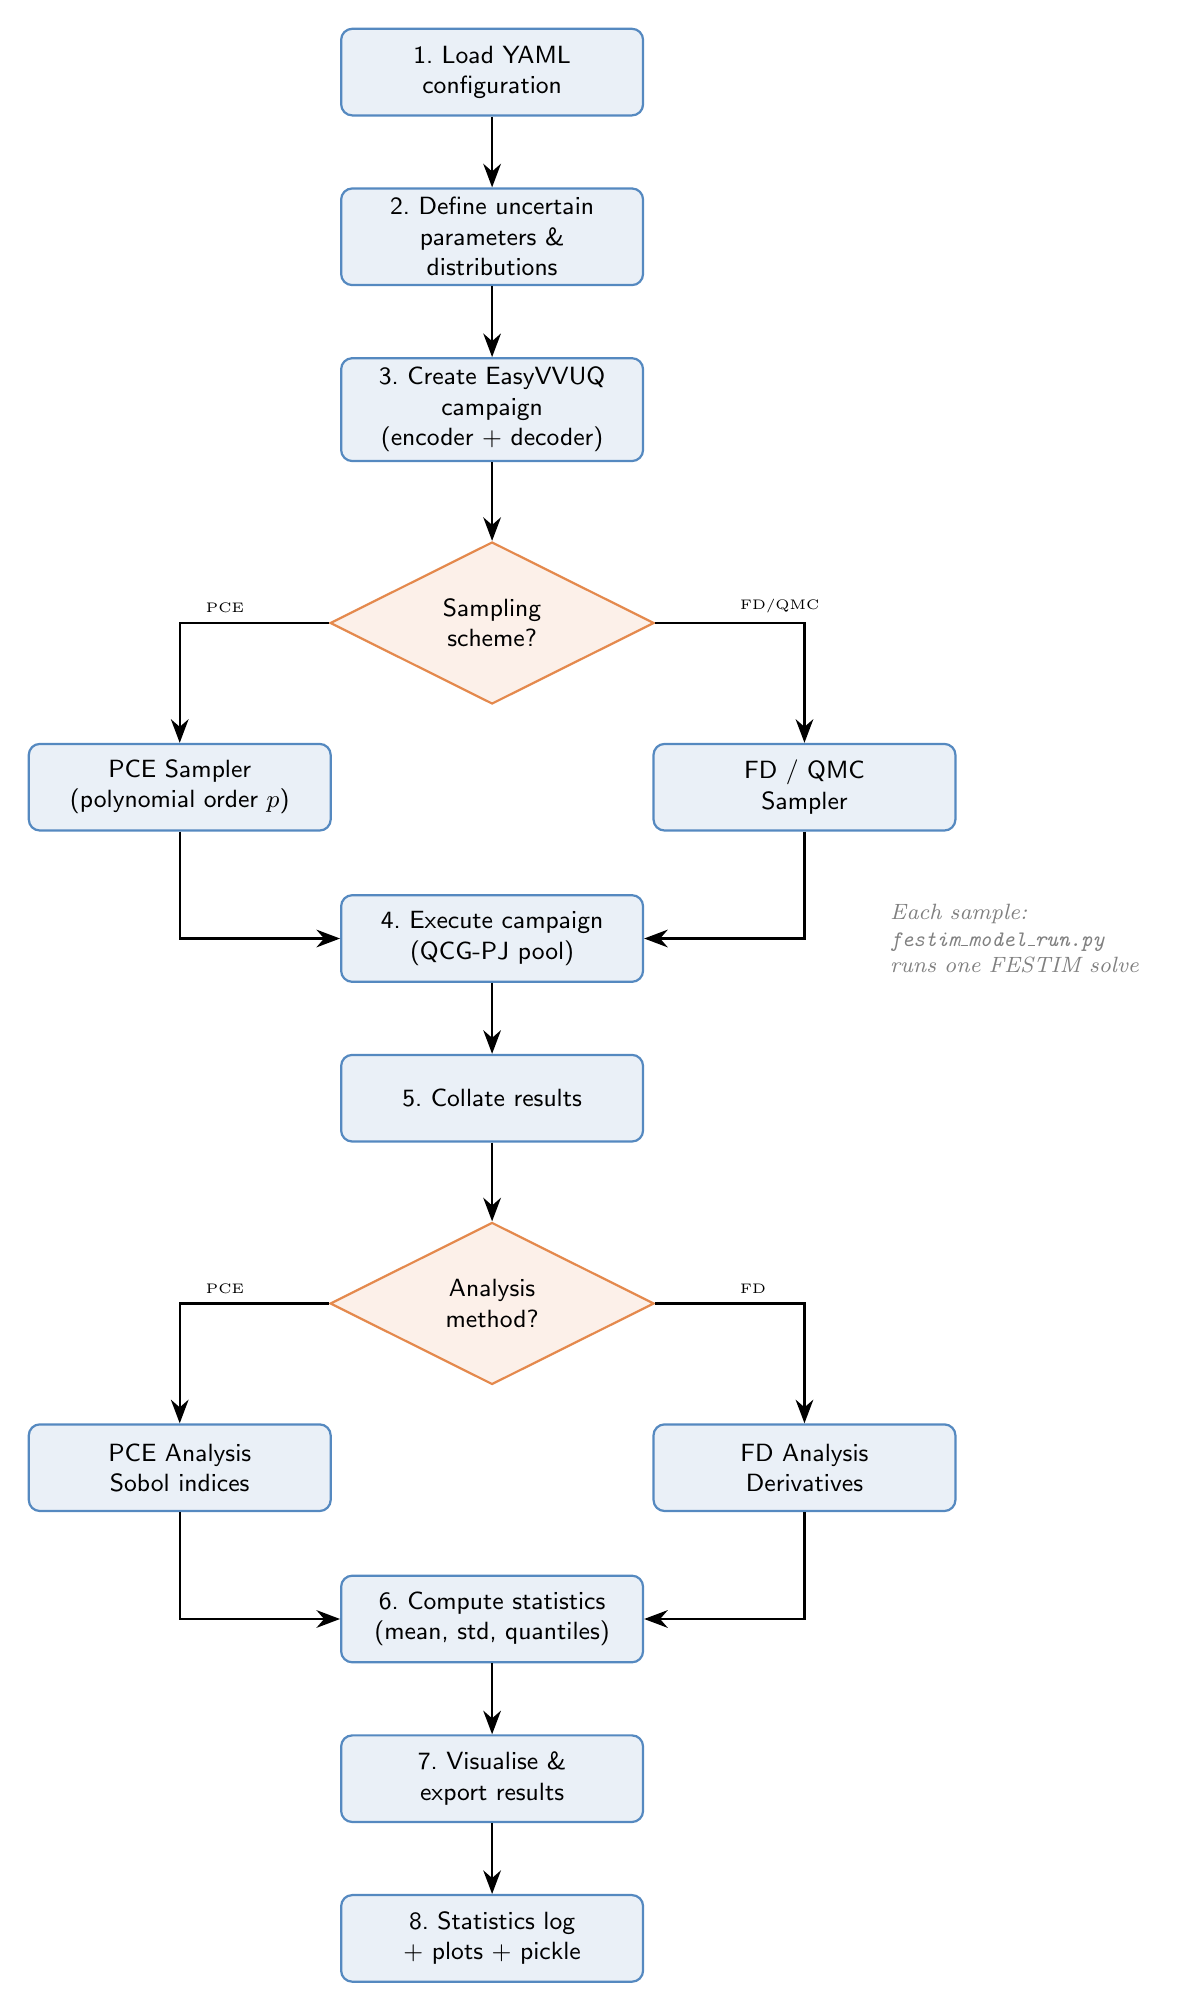
\begin{tikzpicture}[node distance=0.9cm]

% --- Nodes ---
\node[flowbox] (config) {1.\ Load YAML\\configuration};
\node[flowbox, below=of config] (params) {2.\ Define uncertain\\parameters \&\\distributions};
\node[flowbox, below=of params] (campaign) {3.\ Create EasyVVUQ\\campaign\\(encoder + decoder)};
\node[decisionbox, below=1.0cm of campaign] (scheme) {Sampling\\scheme?};
\node[flowbox, below left=1.0cm and 1.0cm of scheme] (pce) {PCE Sampler\\(polynomial order $p$)};
\node[flowbox, below right=1.0cm and 1.0cm of scheme] (fd) {FD / QMC\\Sampler};
\node[flowbox, below=2.4cm of scheme] (execute) {4.\ Execute campaign\\(QCG-PJ pool)};
\node[flowbox, below=of execute] (collate) {5.\ Collate results};
\node[decisionbox, below=1.0cm of collate] (analysis) {Analysis\\method?};
\node[flowbox, below left=1.0cm and 1.0cm of analysis] (pceana) {PCE Analysis\\Sobol indices};
\node[flowbox, below right=1.0cm and 1.0cm of analysis] (fdana) {FD Analysis\\Derivatives};
\node[flowbox, below=2.4cm of analysis] (stats) {6.\ Compute statistics\\(mean, std, quantiles)};
\node[flowbox, below=of stats] (viz) {7.\ Visualise \&\\export results};
\node[flowbox, below=of viz] (report) {8.\ Statistics log\\+ plots + pickle};

% --- Arrows ---
\draw[arrowstyle] (config) -- (params);
\draw[arrowstyle] (params) -- (campaign);
\draw[arrowstyle] (campaign) -- (scheme);
\draw[arrowstyle] (scheme) -| (pce) node[near start, above left, font=\tiny] {PCE};
\draw[arrowstyle] (scheme) -| (fd) node[near start, above right, font=\tiny] {FD/QMC};
\draw[arrowstyle] (pce) |- (execute);
\draw[arrowstyle] (fd) |- (execute);
\draw[arrowstyle] (execute) -- (collate);
\draw[arrowstyle] (collate) -- (analysis);
\draw[arrowstyle] (analysis) -| (pceana) node[near start, above left, font=\tiny] {PCE};
\draw[arrowstyle] (analysis) -| (fdana) node[near start, above right, font=\tiny] {FD};
\draw[arrowstyle] (pceana) |- (stats);
\draw[arrowstyle] (fdana) |- (stats);
\draw[arrowstyle] (stats) -- (viz);
\draw[arrowstyle] (viz) -- (report);

% --- Annotations ---
\node[right=3cm of execute, text width=3.2cm, font=\footnotesize\itshape, text=gray]
  {Each sample:\\
   \texttt{festim\_model\_run.py}\\
   runs one FESTIM solve};

\end{tikzpicture}%
}
\caption{Typical UQ workflow in FESTIM-NIUQ.  The user provides a YAML
  configuration file that defines the physical model and uncertain
  parameters.  EasyVVUQ orchestrates sampling, execution, and analysis.
  Results include statistical moments, Sobol sensitivity indices, and
  publication-quality plots.}
\label{fig:workflow}
\end{figure}


% ============================================================================
\section{Configuration and Usage}
\label{sec:usage}
% ============================================================================

All model and UQ settings are specified in a single YAML configuration
file.  A minimal invocation for independent-parameter UQ is:

\begin{lstlisting}[language=bash]
cd uq
python3 easyvvuq_festim.py --config config/config.uq_test_cj1959.yaml \
        --uq-scheme pce --p-order 2
\end{lstlisting}

\noindent For correlated-parameter UQ with a covariance scan:

\begin{lstlisting}[language=bash]
python3 covariance_influence_analysis.py \
        --config config/config.uq_test_cj1959.yaml \
        --scale log --n-points 5 --p-order 3
\end{lstlisting}

\noindent Postprocessing a completed campaign:

\begin{lstlisting}[language=bash]
python3 uq_postprocessing.py --runs-dir path/to/runs --config config.yaml
\end{lstlisting}

\noindent Interactive viewer:

\begin{lstlisting}[language=bash]
python3 interactive_run_viewer.py --runs-dir path/to/runs -o viewer.html
\end{lstlisting}


% ============================================================================
\section{Draft Notes and Questions Requiring Clarification}
\label{sec:questions}
% ============================================================================

This section collects open questions and items that require input from the
authors or domain experts before finalising the appendix.

\begin{enumerate}
  \item \textbf{Scope of the appendix:}  Should this appendix be
    self-contained (reproducible without reading other documents), or is
    it intended as a supplement to a specific paper or thesis?

  \item \textbf{Physical model details:}
    \begin{itemize}
      \item What is the primary application/material system
            (e.g.\ Li$_2$TiO$_3$ breeding blanket, tungsten PFC, other)?
            % Consider using the mhchem package (\ce{Li2TiO3}) for chemical formulas
      \item Are surface recombination BCs ($k_{r0}$, $E_{k_r}$) actively
            used in the current test cases, or are they placeholder
            functionality?
      \item Is trapping (energy $E_k$, Boltzmann weighting) currently used
            in any published configuration?
    \end{itemize}

  \item \textbf{Parameter distributions:}
    \begin{itemize}
      \item Should the table list specific nominal values and CoVs from a
            reference test case, or remain generic?
      \item Are the uniform and normal distributions the only ones used in
            practice?  The code includes placeholders for log-normal, beta,
            gamma, and exponential.
    \end{itemize}

  \item \textbf{Correlated UQ:}
    \begin{itemize}
      \item What physical justification exists for the correlation between
            $D_0$ and $\kappa$?  Should we cite a specific source?
      \item The Bayesian inverse UQ module
            (\texttt{bayesian\_inverse\_uq.py}) is referenced in the
            memory bank but not found in the repository.  Should it be
            documented or is it on a separate branch?
    \end{itemize}

  \item \textbf{FESTIM version:}
    \begin{itemize}
      \item The code supports both FESTIM~1.4 (\texttt{Model\_legacy}) and
            2.0 (\texttt{Model}).  Should both be documented equally, or
            is v1.4 deprecated?
      \item The steady-state coupled model (tritium + heat) raises
            \texttt{NotImplementedError}.  Should this limitation be noted?
    \end{itemize}

  \item \textbf{QoI definitions:}
    \begin{itemize}
      \item The ``total tritium trapping'' QoI (Boltzmann weighting with
            $E_k$) appears in the memory bank but the corresponding code
            (\texttt{\_compute\_total\_tritium\_trapping}) was not located.
            Please confirm if this is implemented.
      \item What are the units of tritium inventory in a spherical domain?
            Currently documented as $\mathrm{m^{-3}\!\cdot\!m^3}$
            (dimensionless count), but this should be clarified.
    \end{itemize}

  \item \textbf{Diagrams:}
    \begin{itemize}
      \item Should the architecture diagram include the SLURM submission
            scripts (\texttt{uq/slurm\_scripts/})?
      \item Is there a data-flow diagram or class-hierarchy (UML) diagram
            that should be included?
    \end{itemize}

  \item \textbf{Notation and conventions:}
    \begin{itemize}
      \item Should $k_B$ denote Boltzmann's constant in
            $\mathrm{J\,K^{-1}}$, or should $E_D$ be in
            $\mathrm{J\,mol^{-1}}$ with $R$ (gas constant)?  The code
            uses eV in some places and J/mol in others.
      \item Should we include a nomenclature / list of symbols section?
    \end{itemize}

  \item \textbf{References:}
    \begin{itemize}
      \item Which publications should be cited for the FESTIM code, the
            EasyVVUQ framework, and the specific test cases?
      \item Is there a DOI or repository reference for the FESTIM-NIUQ
            package itself?
    \end{itemize}

  \item \textbf{Formatting preferences:}
    \begin{itemize}
      \item Should this be a stand-alone document or an
            \texttt{\\appendix} section within a larger document?
      \item Any journal or style-guide requirements (e.g.\ Elsevier,
            Springer, IEEE)?
    \end{itemize}
\end{enumerate}

% ============================================================================
% END
% ============================================================================

\end{document}
